%
% This chapter provides history of TTM and gives the nod to volunteers and
% supporting organizations
%

\chapter[Welcome]{Welcome to the Moon, Traveler!!!}

% Welcome 

% What is To the Moon?
% History?
% This is true if only doing the flight manual, not the pre-flight
\ifisflight
  % This one page needs to be one column to look right, even
  % in the flight manual, proper.
  % failed experiment to add thumb guides
%   \addthumb{Welcome}{}{white}{black}
\putchapterthumb
\fi

\section*{Mission}
A Burn is a  multi day art and music camping event the intent of which is to build like minded community and to share:
your time, food, gifts, art, love, toys, and talents and participate in creating something in the process that inspires beyond measure.

"A unique and distinctive culture emerges from "The Burning Man" Experience. Rooted in the values expressed by the Ten Principles, this culture is manifested around the globe through art, communal effort, and innumerable individual acts of self expression. To many, it's a way of life." -Burning Man

\subsection*{To The Moon}
Burns reconnect one to their inner child and Merkabah, the divine light vehicle used to tune into the far realm of possibility and innovation.

Embark with us on a journey to the outer rims of creativity, art, music, and community as we initiate a collective experience geared towards positive transformation, endless inspiration, and participatory
co-creation. Bring your SELF, your talents, your radical self-expression, and your stardust TO THE MOON and back as we travel together further than our own imagination. You get out of it what you put int.

Simply put, we play with fire and run with scissors in a space shaped by our fantasy and that which is conjured up by our inspiration and elbow grease.... the sky is the limit. 

\subsection*{...And Back}
Art, Participation, Fire Play, Music and so much more motivate this 
community to build a temporary dwelling in which there is no stranger nor are there spectators. Everybody pitches in and brings something to the table.  
We stare at the clouds, dream in dust, set fire to the rain and howl at the moon.  

A Burn is an incredible way of learning firsthand the experience of the Whole being greater than the sum of its parts.  

It's a place where participants gather to celebrate self-expression and community who happen to know how to throw a party.  They conceive and build interactive theme camps, art installations, mutant vehicles, costumes and performances, and they gift them for the benefit and enjoyment of each other!

Art Camps, Theme Camps, Sounds Camps all are an integral part and at the heart of this experience.  The event comes to a climax with the burning of the Effigy Saturday night, and usually ends after Sunday's Temple Burn. 

The culture rallies around causes and activism from local art exhibits to food and coat drives to Burners Without Borders - spearheading change, inspiring involvement and making a splash! 

"In Dust we trust....."


\vspace*{\fill}
\begin{figure}[!h]
\centering
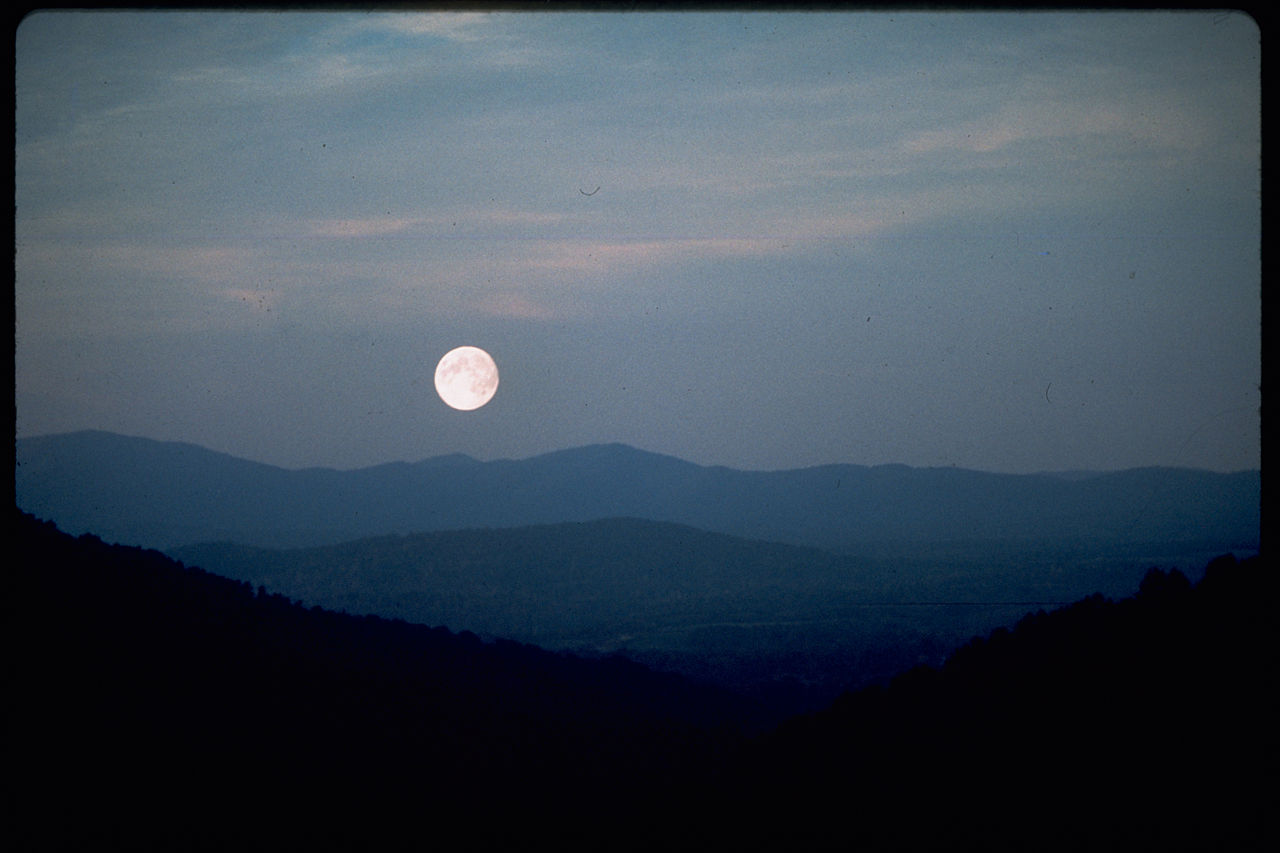
\includegraphics[width=.8\textwidth, trim=10 0 50 0, clip]{images/ShenandoahMoon}
% \caption{}
\label{image:mountainmoom}
\end{figure}
\vspace*{\fill}
